
\section{Data}
\label{supp_sec:data}

This section describes the set of leaf and cre-line experimental combinations.

\newpage

\begin{figure}[H]
    \centering
    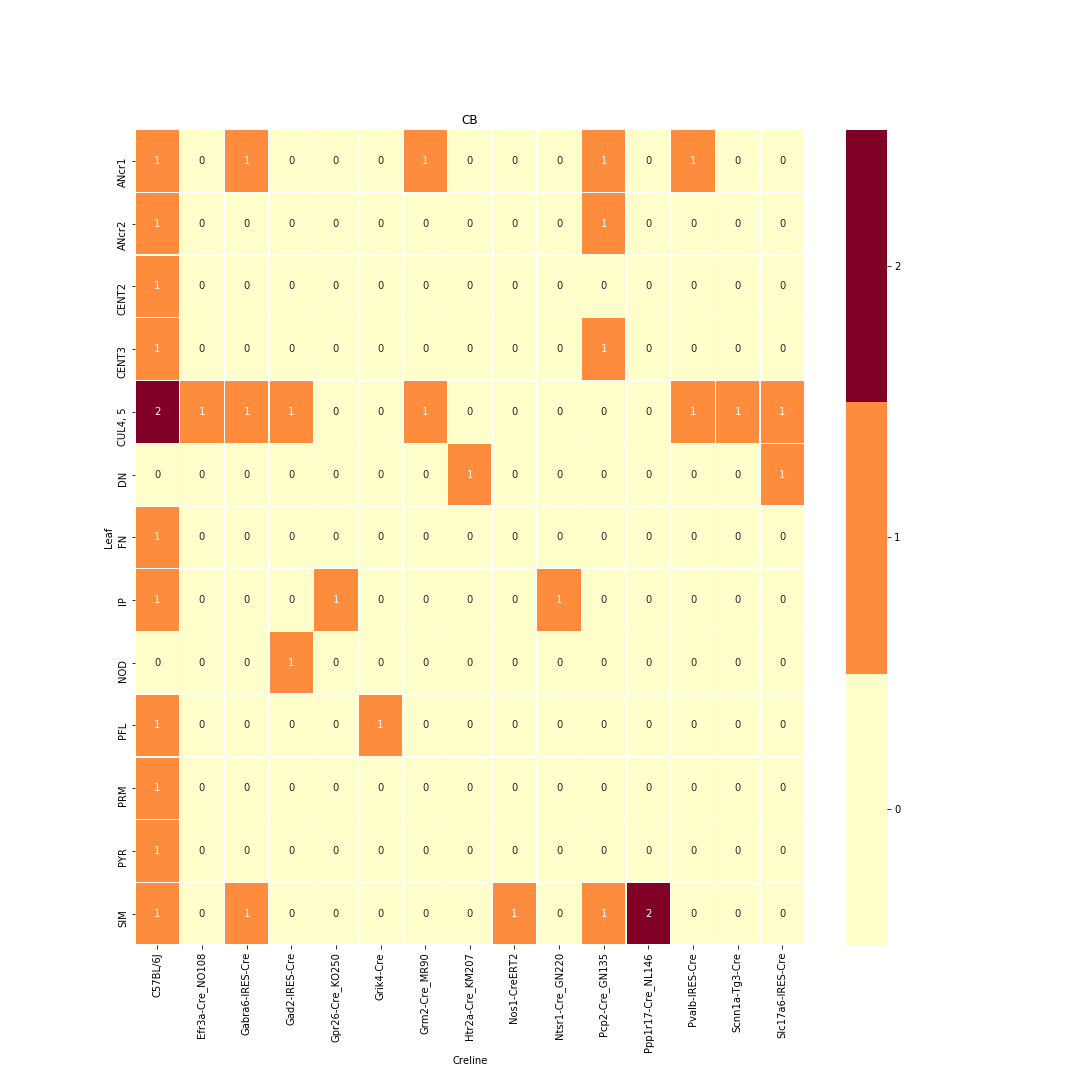
\includegraphics[width = 7in]{figs/CB centroid densityoct12.png}
    \label{fig:my_label}
\end{figure}
\newpage

\begin{figure}[H]
    \centering
    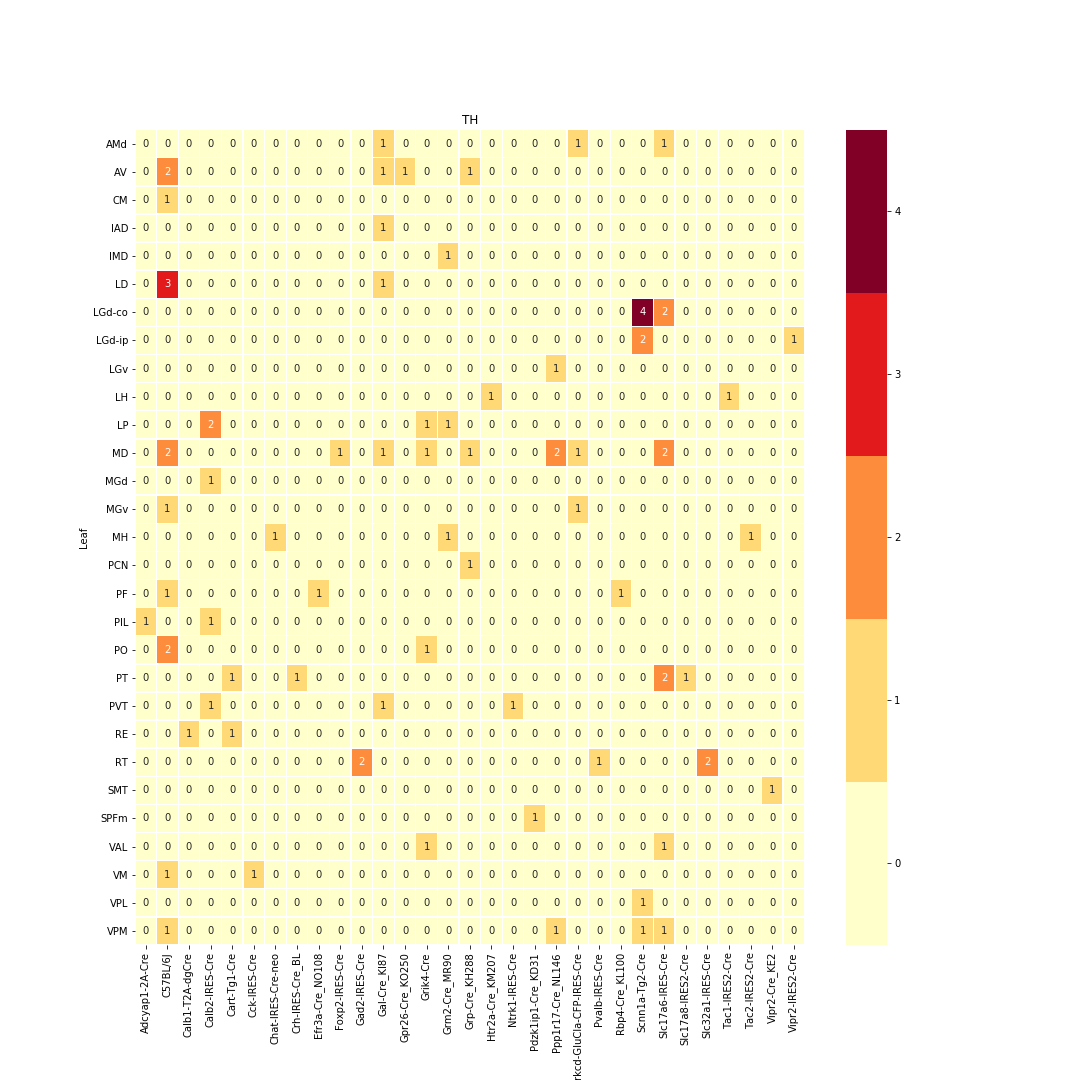
\includegraphics[width = 7in]{figs/TH centroid densityoct12.png}
    \caption{Caption}
    \label{fig:my_label}
\end{figure}
\newpage

\begin{figure}[H]
    \centering
    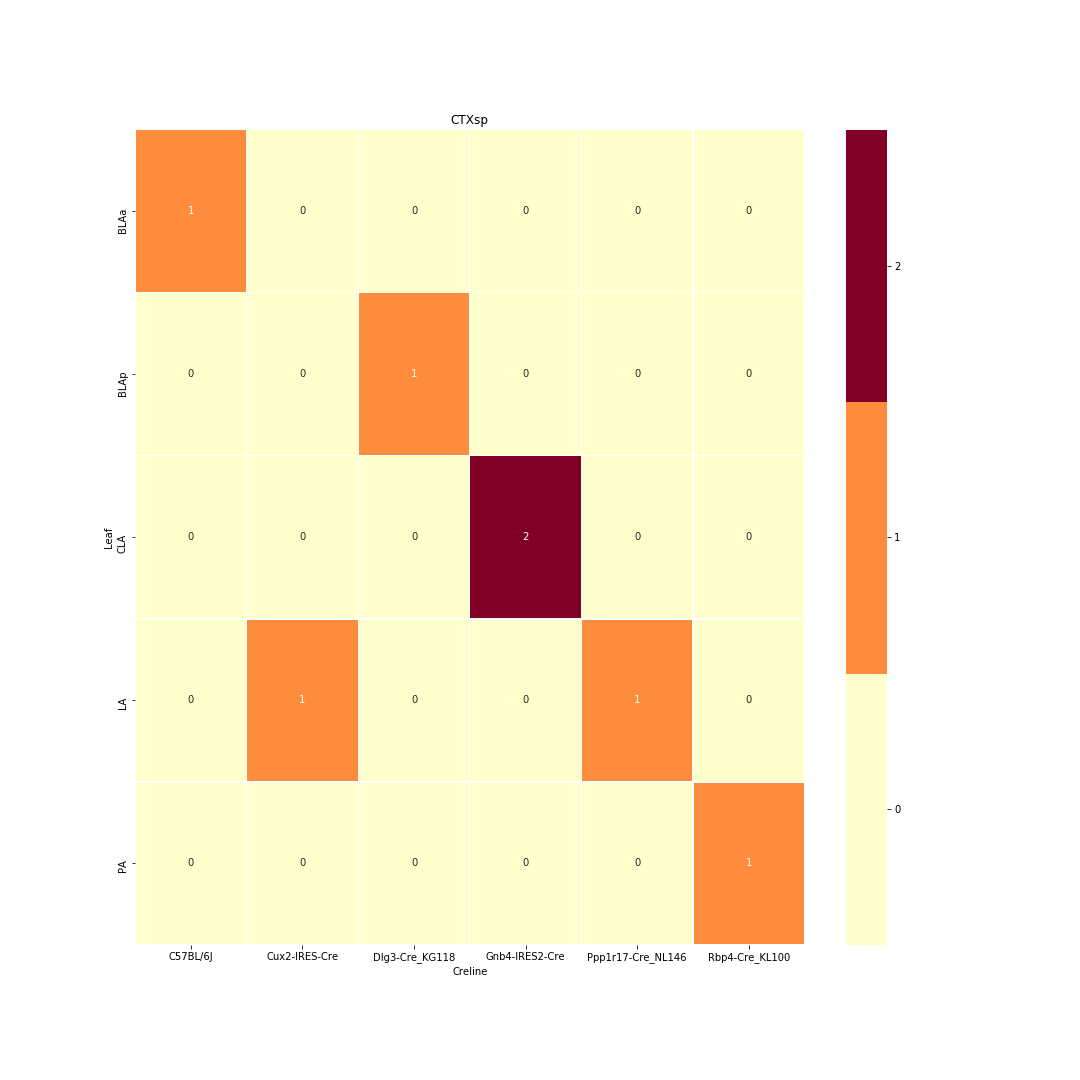
\includegraphics[width = 7in]{figs/CTXsp centroid densityoct12.png}
    \caption{Caption}
    \label{fig:my_label}
\end{figure}
\newpage

\begin{figure}[H]
    \centering
    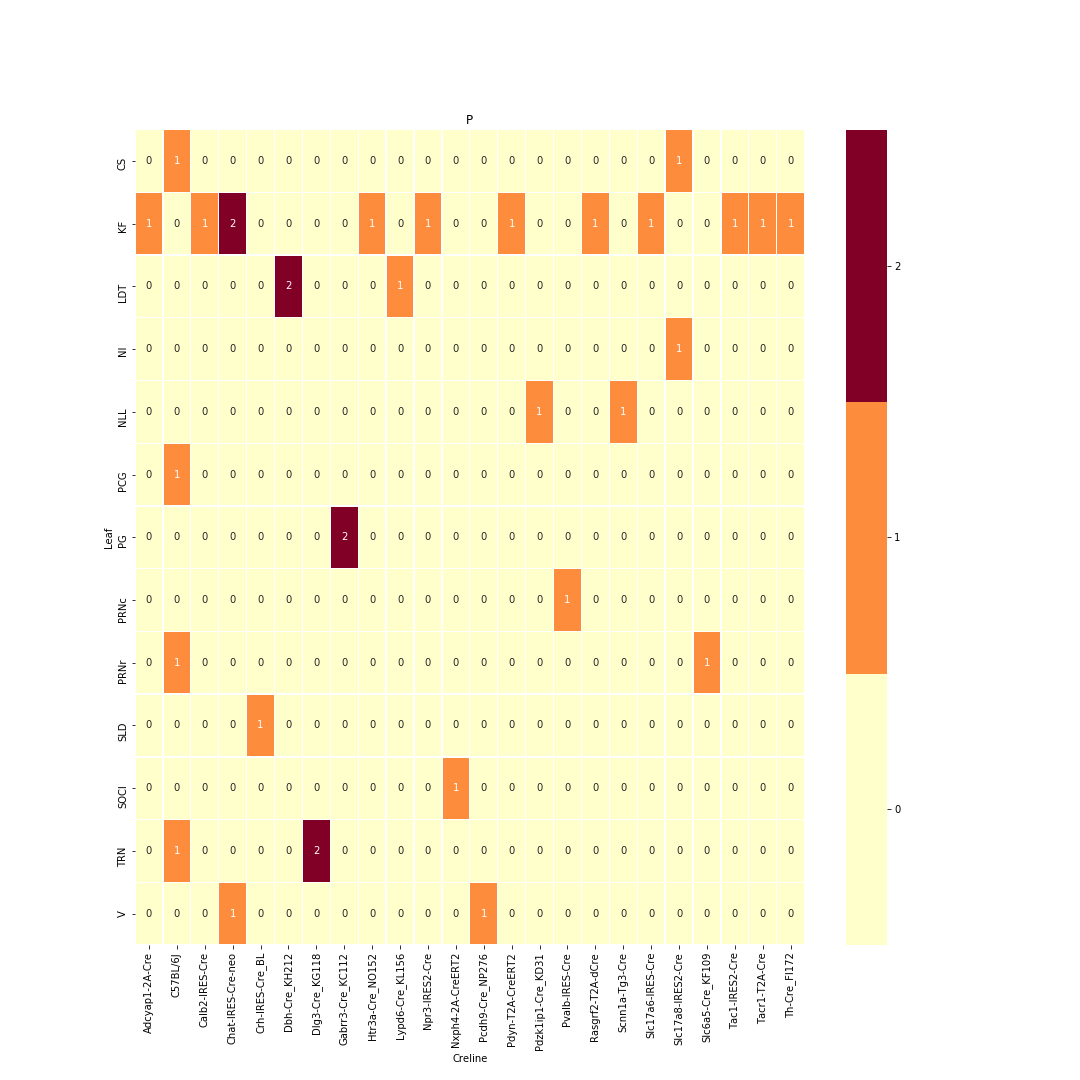
\includegraphics[width = 7in]{figs/P centroid densityoct12.png}
    \label{fig:my_label}
\end{figure}
\newpage

\begin{figure}[H]
    \centering
    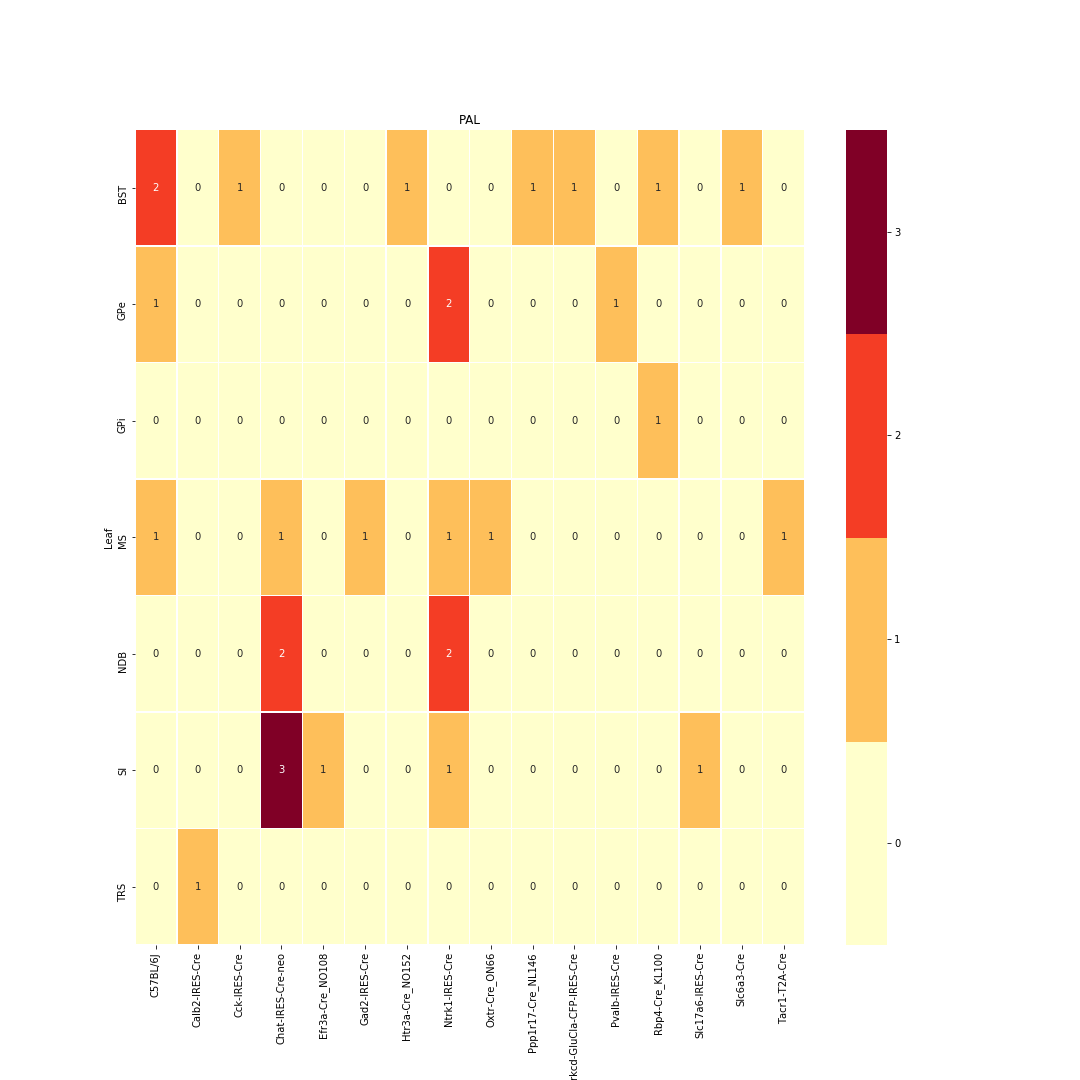
\includegraphics[width = 7in]{figs/PAL centroid densityoct12.png} 
    \label{fig:my_label}
\end{figure}
\newpage

\begin{figure}[H]
    \centering
    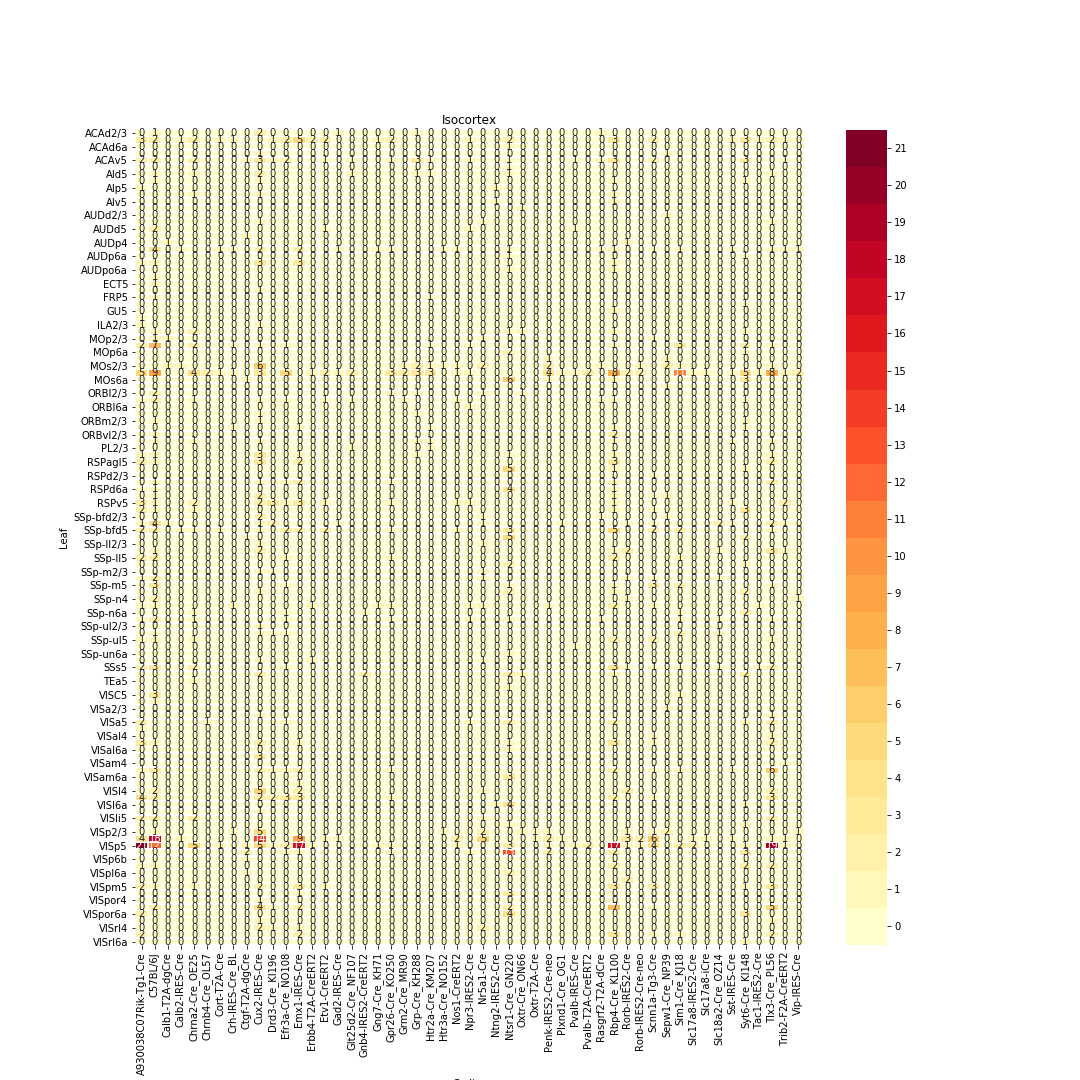
\includegraphics[width = 7in]{figs/Isocortex centroid densityoct12.png}
    \label{fig:my_label}
\end{figure}
\newpage

\begin{figure}[H]
    \centering
    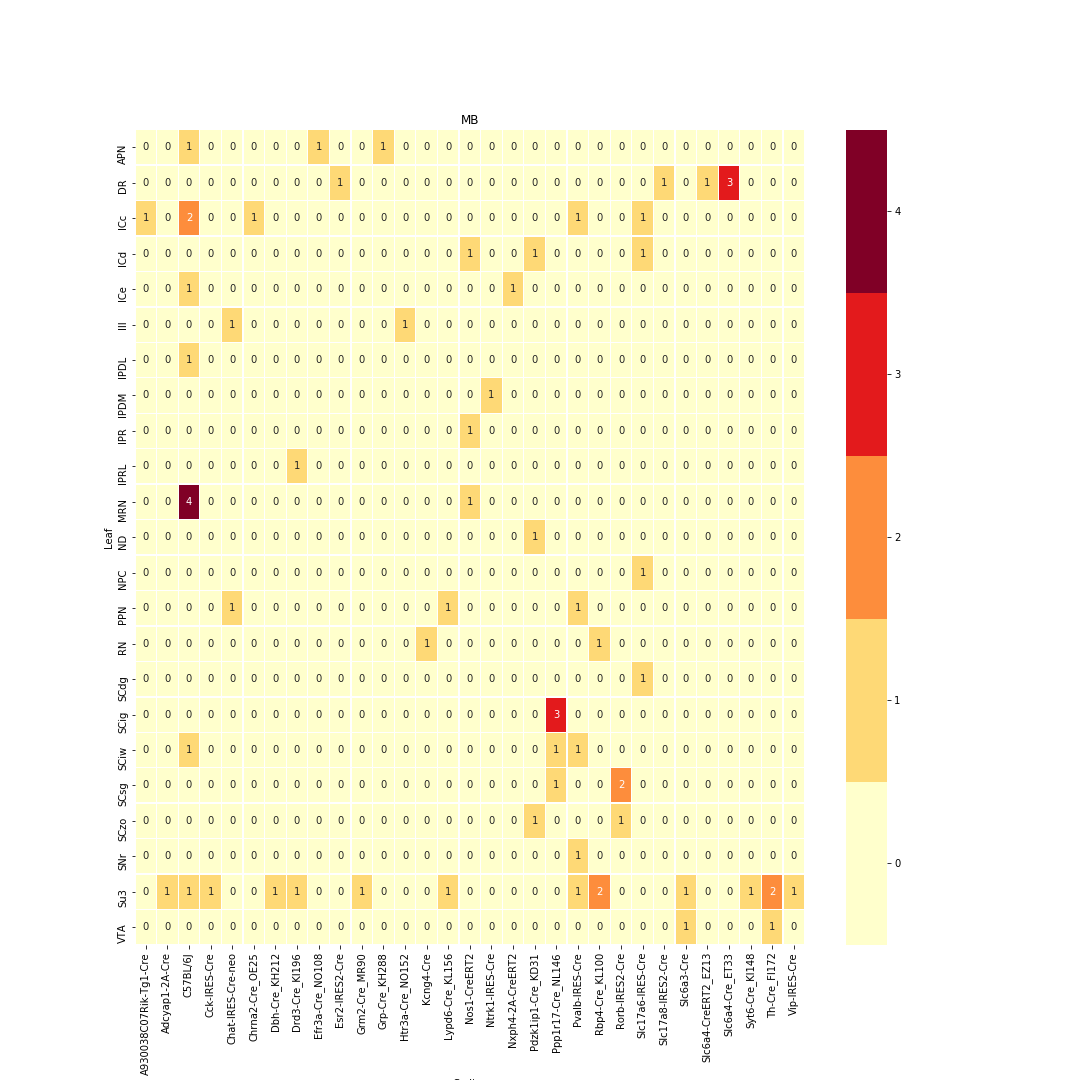
\includegraphics[width = 7in]{figs/MB centroid densityoct12.png} 
    \label{fig:my_label}
\end{figure}
\newpage

\begin{figure}[H]
    \centering
    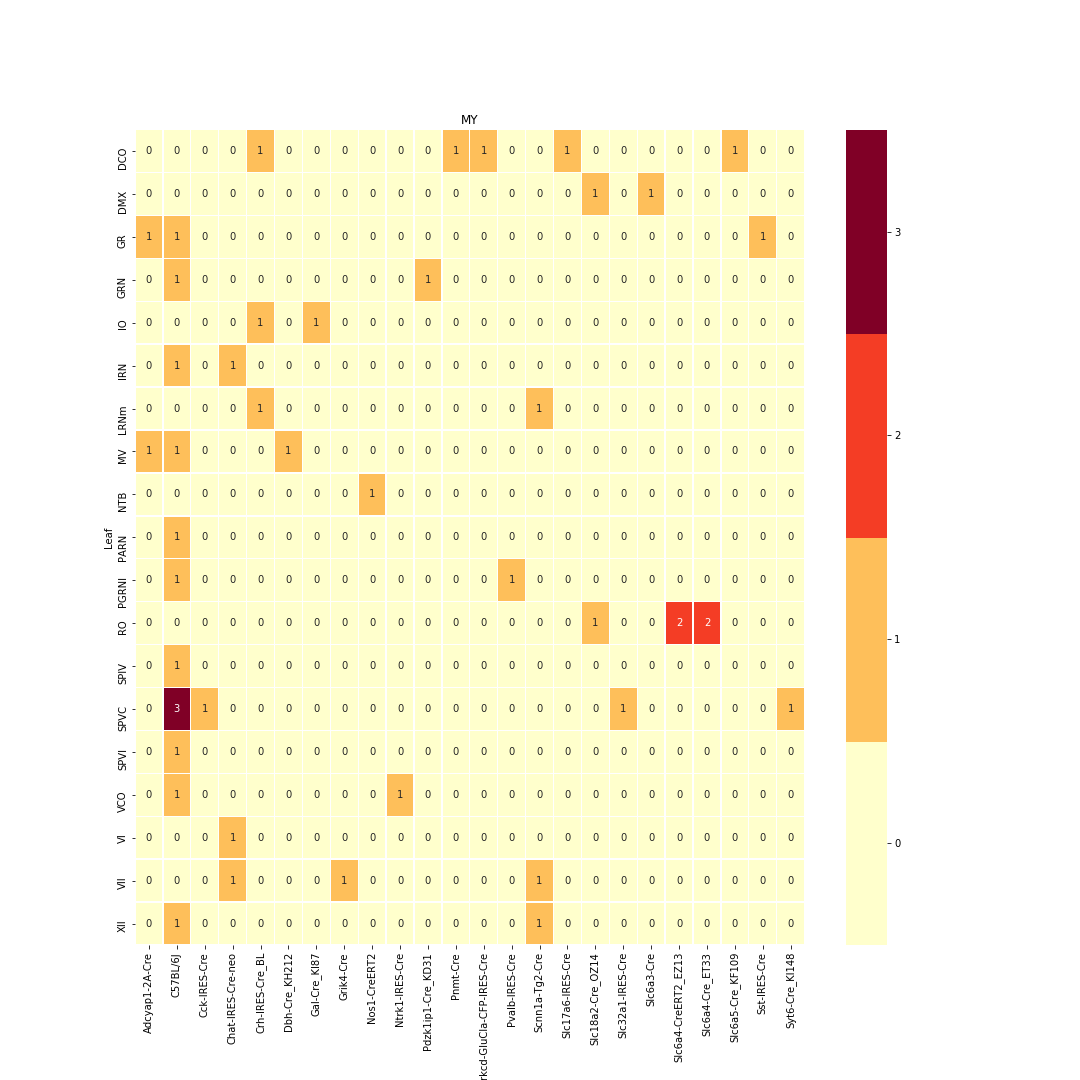
\includegraphics[width = 7in]{figs/MY centroid densityoct12.png} 
    \label{fig:my_label}
\end{figure}
\newpage

\begin{figure}[H]
    \centering
    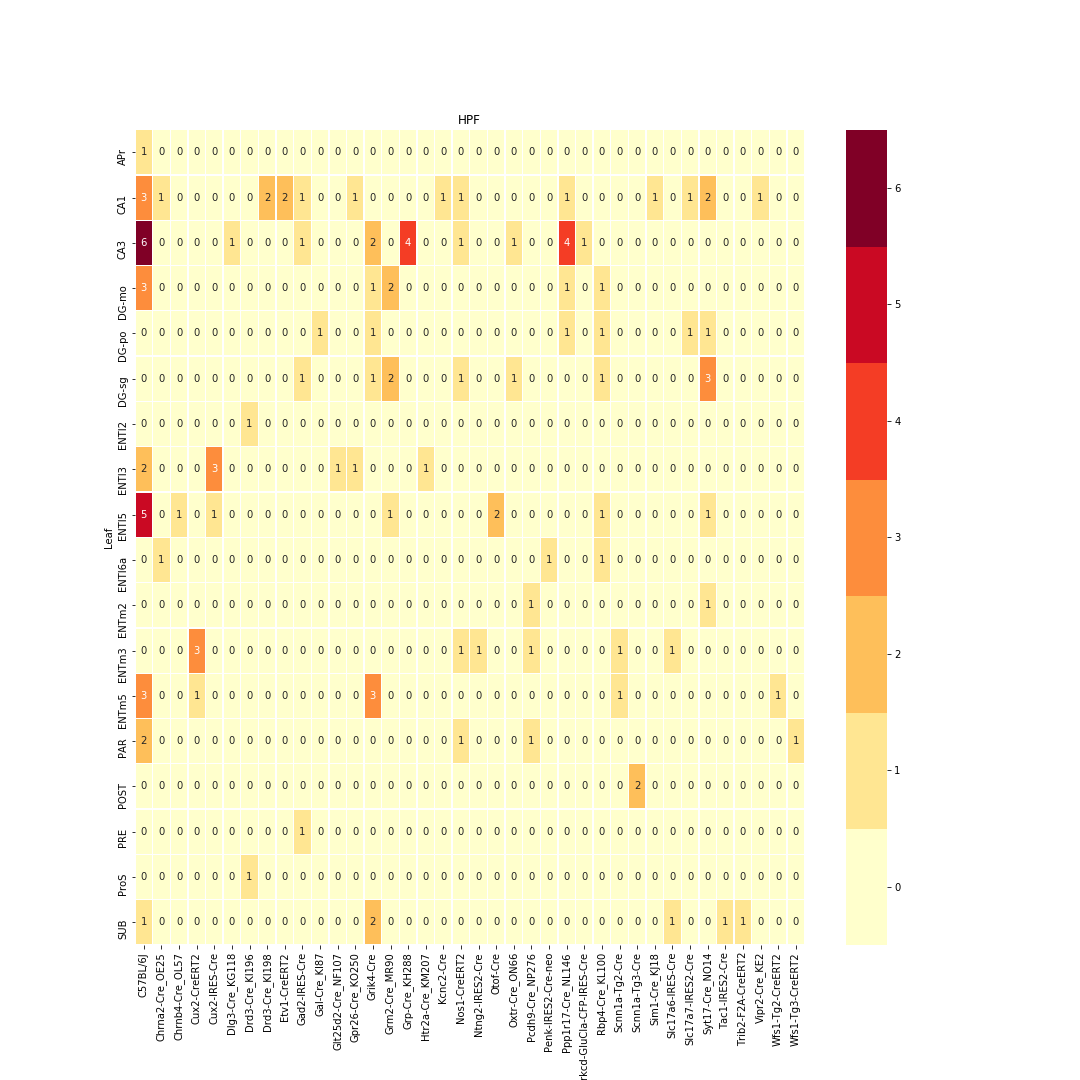
\includegraphics[width = 7in]{figs/HPF centroid densityoct12.png} 
    \label{fig:my_label}
\end{figure}
\newpage

\begin{figure}[H]
    \centering
    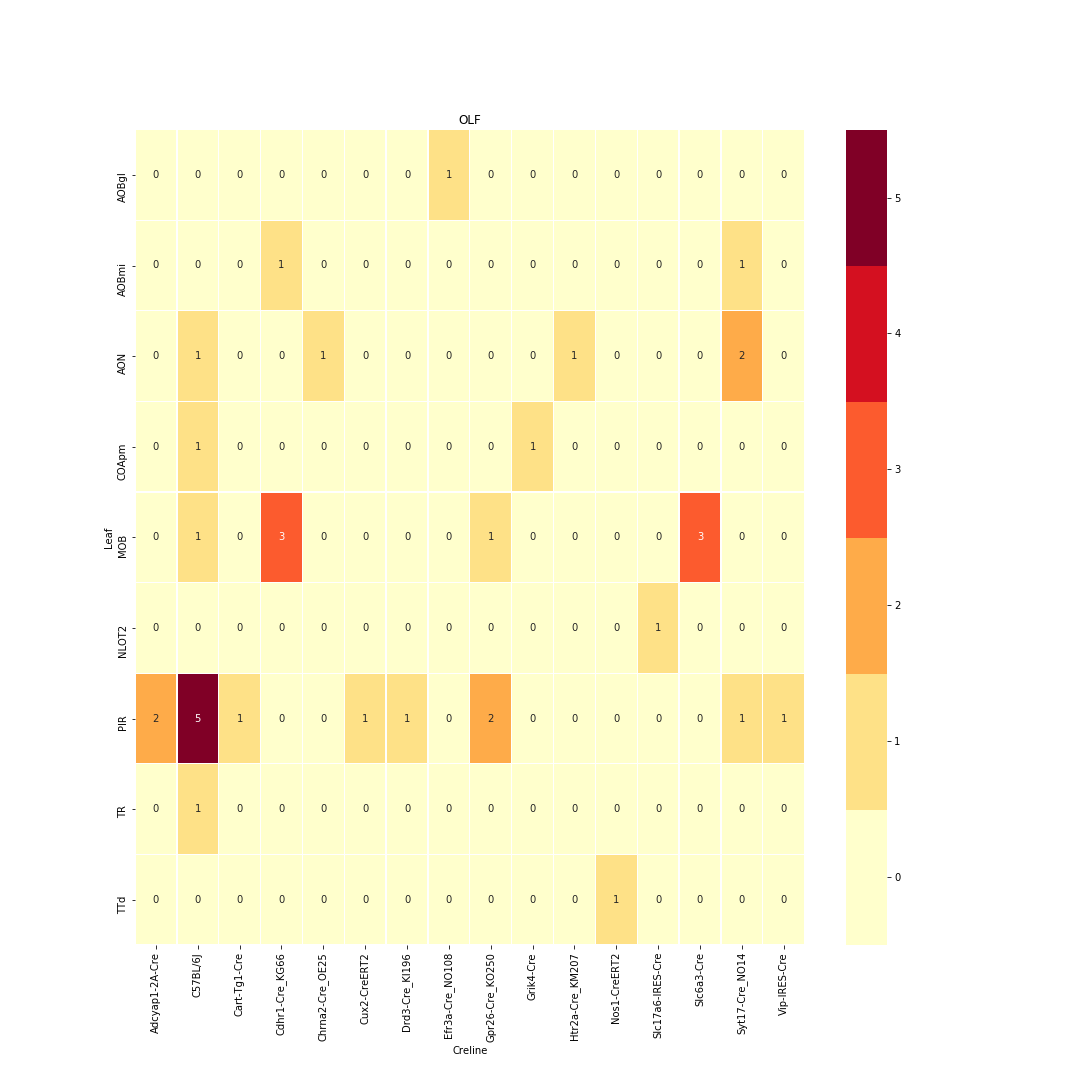
\includegraphics[width = 7in]{figs/OLF centroid densityoct12.png} 
    \label{fig:my_label}
\end{figure}
\newpage

\begin{figure}[H]
    \centering
    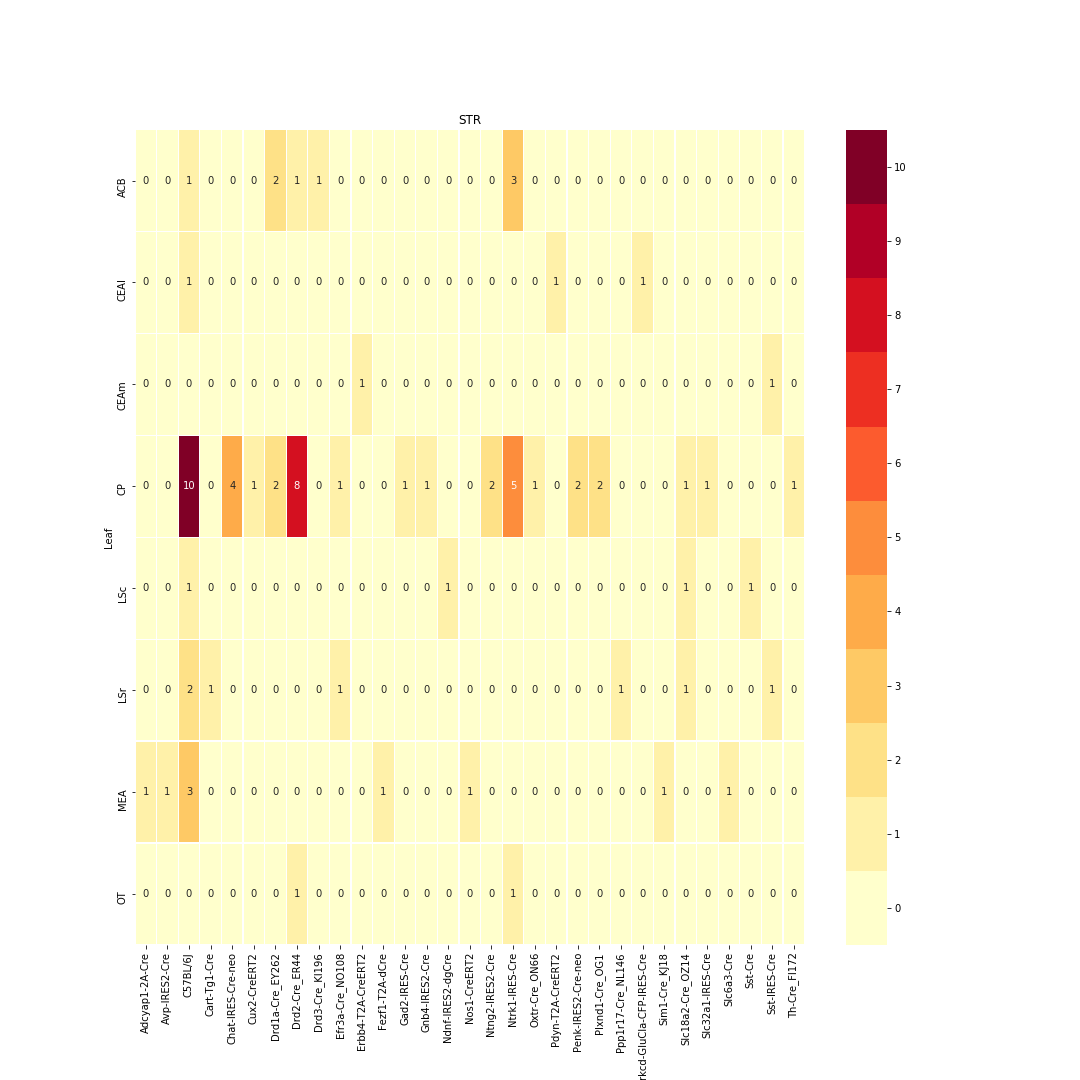
\includegraphics[width = 7in]{figs/STR centroid densityoct12.png} 
    \label{fig:my_label}
\end{figure}
\newpage

\begin{figure}[H]
    \centering
    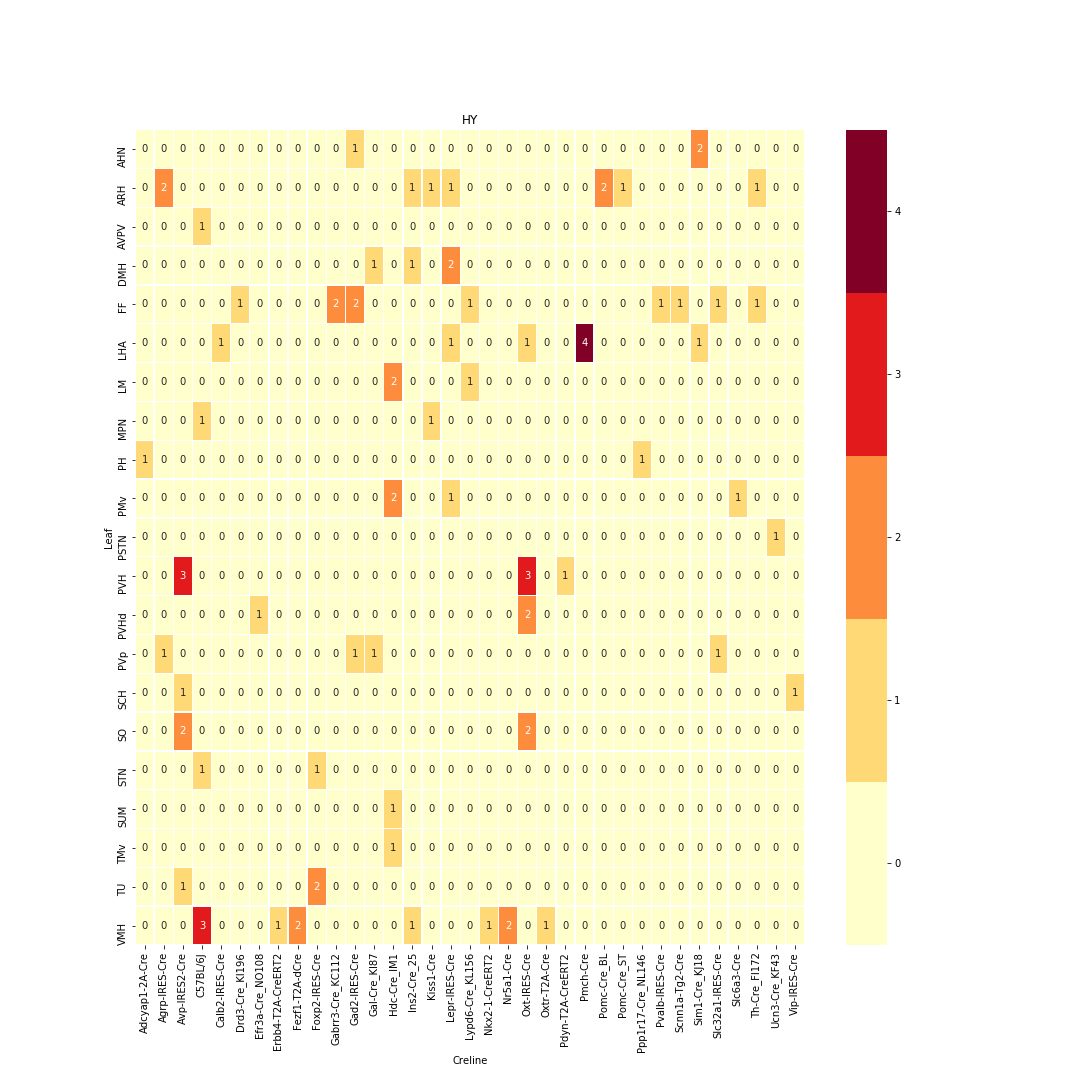
\includegraphics[width = 7in]{figs/HY centroid densityoct12.png} 
    \label{fig:my_label}
\end{figure}

\newpage


\section{Data preprocessing}

%In this paper, source regions are typically at the lowest level (shown in blue).
%In the cortex, layer-specific connectivities are generated.
%Injection mask
%Projection mask
%Data quality mask
%From this, a weighted centroid $c(x_i) \in \mathbb R^3$ and 

%Regionalization occurs in several ways.
%A per-region average $r(x_i) \in \mathbb R^{M_i}$ may be computed, where $M_i$ is the number of substructures in the major brain region.
%Similarly, for the projection, $r(y_i) \in R^{M}$.


\label{sec:dp}

Several data prepreprocessing steps take place prior to evaluations of the connectivity matrices.
Injections and projections were downloaded using the Allen SDK.
These were originally annotated manually.
The injection and projection vectors are Hadamard multiplied by a data quality matrix. We also have a map $A: \mathbb R \to \mathbb R^{|S|}$ where $S$ is the number of structures that takes the average value for voxels in that structure

\begin{algorithmic}
%\label{alg:norm}
%\begin{algorithm}{Injection $x(i)$, Projection $y(i)$, Injection centroid $c(i) \in \mathbb R^3$, injection fraction $F(i)$, data mask $M(i)$}
\State Data-quality censor $y_M (i) = M(i) \odot y(i)$ (also $x_M(i) = M(i) \odot x(i)$ for linear model)
%\State Normalize $x_N(i) = F(i) \odot x_M(i)$ (only for linear model)
%\State Average structures $y_S (i) = A y_M(i)$ (also $x_S (i) = A x_M(i)$ for linear model)
%\State Normalize $\tilde y(i) = \frac{y_S (i)}{\|y_S (i)\|}$ (also $\tilde x (i) = A x_M(i)$ for linear model)
% \Return $\tilde y(i)$ (optional $\tilde x(i)$ )
%\end{algorithm}
\end{algorithmic}

The data-quality censor is established by \skcomment{fill}
The injection fraction accounts for the relatively coarse graining of the voxel grid compared with the histological analysis used to establish the injection region.  In particular, certain voxels are only partially contained within the injection region.

\subsubsection{Normalization}

One basic but significant methodological change from \citet{Knox2019-ot} is the normalization of projection vectors.

\begin{comment}
\begin{figure}
    \centering
    \includegraphics{}
    \caption{Caption}
    \label{fig:my_label}
\end{figure}
\end{comment}
%We also note that normalization simplifies our loss function.
The loss function in \citet{Knox2019-ot} is
\begin{eqnarray*}
\frac{\|y - \hat y\|} {\|y\|\|\hat y\|}
\end{eqnarray*}

%We find the $l2$ norm not appropriate in a few ways 1) there is not a clear inner product structure on the connectome.

%It is reasonable to ask can we back-divide densities after normalization... seemingly yes.  But then how should we interpret the previously normalized row sums.  Areas with high row sum have high density of connection.  

%It doesn't matter if we normalize prior to regionalization as long as we don't correct for density of the target region.
%which, due to normalization, can be rewritten as simply the $l2$ loss $\|y - \hat y\|.$  Note that, due to normalization, $\|y - \hat y\| = \langle y - \hat y , y - \hat y \rangle = 2 - 2 \langle y, \hat y\rangle $, and, applying normalization again, $ \langle y, \hat y\rangle $ is the vector cosine of $\hat y$ and $y$.


\subsection{Estimators}

Our estimators span a range of training and featurization methods.
One commonality is that they model a connectivity vector $f (\mathcal D, v,s)  \in \mathbb R^T$, and so we may write
\begin{eqnarray*}
f (v,s,t) = f (v,t)[t].
\end{eqnarray*}
Thus, for the remainder of this section, we will discuss only $f (s,v)$.

\paragraph{Regionalized non-negative least squares}

In the non-negative least squares approach of \citet{Oh2014-kh}, the injection is considered only through its centroid, while the projection is considered regionalized.
The prediction for a given region is then given by the integral of predictions over that region, which is computed as a sum over voxels.

\paragraph{Centroid-based Nadaraya-Watson}

In the Nadaraya-Watson approach of \citet{Knox2019-ot}, the injection is considered only through its centroid, while the projection is considered regionalized.
The prediction for a given region is then given by the integral of predictions over that region, which is computed as a sum over voxels.
That is,
\begin{eqnarray*}
f_*({\mathcal D}_i) = \{c(x_i) , r(y_i)\}.
\end{eqnarray*}
Since the injection is considered only by its centroid, this model only generates predictions for particular locations $c$.  The prediction for a structure $s$ is given by integrating over locations within the structure.
That is,
\begin{eqnarray*}
\label{eq:regionalize}
f^* (\hat f (f_*(\mathcal D))) (v,s) = \sum_{c \in s} \hat f (f_*(\mathcal D)) (v,c).
\end{eqnarray*}
Here, we set $\hat f$ to be the so-called Nadaraya-Watson estimator
\begin{eqnarray*}
\hat f_{NW}( c(x_{1:n}) , r(y_{1:n}) ) (c,v) =  \sum_{i \in I} \frac{ \omega_{c(x_i) c}}{\sum_{i \in I} \omega_{c(x_i) c}} r(y_i)
\end{eqnarray*}
with $\omega_{c(x_i) c} = \exp( - \gamma d( c , c(x_i))^2 )$ where $d$ is the Euclidean distance between centroid $c(x_i)$ and voxel $c$.
%\begin{eqnarray*}
%f^*( f_*(\mathcal D), v,s) = \sum_{c \in s} f_{NW}^{ \gamma} (c, c(x_{I}) , r(y_{I}), v).
%\end{eqnarray*}

Several facets of the estimator are visible here. $f_{NW}^{\gamma}$ is the Nadaraya-Watson estimator with smoothing given by inverse-bandwidth $\gamma$.
A smaller $\gamma$ corresponds to a greater amount of smoothing, and index set $I \subseteq  \{1:n\}$ indicates which experiments to use to generate the prediction.
Fitting $\gamma$ via empirical risk minimization therefore bridges between $1$-nearest neighbor prediction and averaging of all experiments in $I$.
In \citet{Knox2019-ot}, $I$ consisted of experiments sharing the same brain division.
This model is easily extensible to a cre-specific model by restricting the index set to only include experiments with the same cre-line.

%The model is then a weighted sum of nearby centroids.
%\begin{eqnarray*}
%f_{NW} (c, c(x_{1:n}) , r(y_{1:n}), v,t) &= \sum_{i \in I} %\tilde w_c r(y(i))
%( \tilde w_c^R)^T y_{1:n, t}
%\end{eqnarray*}
%with 
%\begin{eqnarray*}
%w_{ci} = \exp( - \gamma \| c - c(i)\|_2^2 ) \\
%\tilde w_{ci^R} = \frac{w_{ci} }{\sum_}
%\end{eqnarray*}

%\begin{eqnarray*}
%f_{NW} (c, c(x_{1:n}) , r(y_{1:n}), v,t) = ((1_v^n)^T \tilde w_c)^T y_{1:n, t}
%\end{eqnarray*}
%where $(1_{v,M}^n)$ is a vector of length $n$ indicating %only using experiments with the same cre-line and major structure.

%
\paragraph{The expected-loss estimator}

The response induced by each of the cre-lines is effected by both the injection location and the targeted cell types.
Cre-lines that target similar cell types are therefore expected to induce similar projections, and including similar cre-lines in our estimator thus increases the effective sample size.
In order to leverage this fact in a data-driven way, we introduce an estimator that assigns a predictive weight to each training point that depends both on its centroid-distance and cre-line.
This weight is determined by the expected prediction error of each of the two feature types, as determined by cross-validation.
These weights are then utilized in a Nadaraya-Watson estimator in a final prediction step.

%
%standard optimization approach gives plane
We formalize cre-line behavior as the average regionalized projection of a cre-line in a given leaf.
This vectorization of categorical information is known as target encoding.
We define a {\textit cre-distance} in a leaf to be the distance between the target-encoded projections of two cre-lines.
The relative predictive accuracy of cre-distance and centroid distance is determined by fitting a surface of projection distance as a function of cre-distance and centroid distance. 


%centroids are weighted more highly in the centroid-based Nadaraya-Watson estimator.
%this estimator is an average (limit) of the cre-specific NW



In mathematical terms, our full feature set consists of the centroid coordinates and the target-encoded means of the combinations of virus type and injection-centroid structure.
That is, 
\begin{eqnarray*}
f_*({\mathcal D}_i) = \{c(x_i) , \bar r(y_{I_v}), r(y_i) \}.
\end{eqnarray*}
$f^*$ is defined as in \eqref{eq:regionalize}. The expected loss estimator is then 
\begin{eqnarray*}
\hat f_{EL} (c, c(x_i),v , r(y_{I_v})) =  \sum_{i \in I} \frac{ \nu {(c(x_i) , c, v_i, v)}}{\sum_{i \in I} \nu {(c(x_i) , c, v_i, v) }} r(y_i)
\end{eqnarray*}
where
\begin{eqnarray*}
\nu_i = \exp (- \gamma g( d(c, c(x_i))^2, d(\bar r (v), \bar r (v_i))^2))
\end{eqnarray*}
Note that $g$ must be a concave, non-decreasing function of its arguments with with $g(0,0) = 0$, then $g$ defines a metric on the product of the metric spaces defined by experiment centroid and target-encoded cre-line, and $\hat f_{EL}$ is a Nadaraya-Watson estimator.  A derivation of this fact is given in Appendix \ref{supp_sec:el}, and we therefore use shape-constrained B-splines to estimate $g$.

This contrasts with the model is \citet{Knox2019-ot}, where $\hat f(c)$ does not depend on $v$, and \citet{Oh2014-kh}, where connectivity was directly estimated by $\hat f$ a function of $S$ without an integral.
Estimating $\hat f(v, c)$ shares the advantage of fine-scale spatial resolution with \citet{Knox2019-ot}, but in addition enables us to model a particular virus-type $v$, and, as we will see, make use of experimental data in our estimator.


%We fit $g$ using a simple heuristic based.
%Since we wish to weight similar points more highly, we weight distances in cre-space and centroid-space by how well they predict the response variable.
%Due to the fact that the cre-space is defined with respect to the response variable, points are removed from their cre-mean prior to cross-validation.
%Figure shows an example of such an estimated $g$.

%Theoretically, there is a trade off between similarity of the point, and the statistical convergence.
%In the low-sample size setting, it is worth utilizing points from similar groups.


%All of these methods are improvements on the average method.

%is the set of ipsilateral and medialateral brain regions, $R_{IMC}$ is the set of ipsilateral, mediolateral, and contralateral targets,

%We use the experiments to estimate the virus-specific connectivity matrix $\mathcal C_v \in \mathbb R^{|R_{IM}| \times |R_{IMC}|}$.
%$R_{IM}$ is the set of ipsilateral and medialateral brain regions, $R_{IMC}$ is the set of ipsilateral, mediolateral, and contralateral targets, and $v$ is a cre-line. 

%Each row of this matrix represents the fraction of projected virus to a structure $r$.

%Given a region $r$, we estimate the projection vector ${\mathcal C_v}_r$, the row corresponding to the region, both $v$ and the spatial position of $r$.

%This estimate is 
%\begin{equation}
%\hat {C_v}_{r} = \sum_{c \in r} \hat y (v, c) dc.
%\end{equation}
%Here, $\hat y(v, c)$ is the estimate projection pattern of virus-type $v$ at spatial position $c$ within structure $r$.
%In our experiments, this sum is discretized at the voxel level.


%Given a centroid position $c$ and cre-line $v$, we call %our estimator of the projection $\hat y(v, c)$, which is the local weighted average
%\begin{align*}
%\hat y(v, c) &= \sum_{i \in R(c)} \tilde w_\gamma(v,c,c(i),v(i)) y_i
%\end{align*}
%with
%\begin{align*}
%    \tilde w_\gamma(v,c,c(i),v(i)) &= \frac{w_\gamma(v,c,c(i),v(i))}{\sum_{i \in R(c)} w_\gamma(v,c,c(i),v(i))} \\
%\end{align*}
%In this average, nearby experimental projections $y_i$ are averaged with weights determined with respect to the cre-lines $v(i) \in C$ and injection centroid positions $c(i) \in \mathbb R^3$ in the training data.
%In contrast with the estimator in \citet{Knox2019-ot}, we define these weights to depend on cre-line as well as centroid positions.
%In particular,
%\begin{align*}
%    w_\gamma(v,c,c(i),v(i)) &= \exp(- \gamma \hat l ( \Delta c_i,\Delta y_v (i))) % \bar y_{r(c)} (v(i)) - \bar y_{r(c)} (v)) )
%\end{align*}
%where, defining 
%\begin{align*}
%\Delta c_i &= c(i) - c \\
%\Delta y_v (i) &= \bar y_{r(c)} (v(i)) - \bar y_{r(c)} (v) \\
%\delta c_i &= \|\delta c_i\|_2^2 \\
%\delta v_i &= \|\Delta y_v (i)\|_2^2
%\end{align*}
%we have
%\begin{align*}
%&\hat l (\Delta c_i, \Delta y_v (i)) = \sum_{r \in R(c)} \sum_{j,k \in r} \frac{w_{\gamma'}'( \delta c_{jk} ,\delta c_i, \delta v_{jk} , \delta v_i)}{1} \|y_j - y_k\|_2^2 
%= \|y_i - y_j\|
%\| c - c(i) \|_2^2, \|\bar y(v, r(c)) - \bar y(v(i))\|_2^2)
%\end{align*}
%where
%\begin{align*}
%w_{\gamma'}'( \delta c_{jk} ,\delta c_i, \delta v_{jk} , \delta v_i) &= \exp(- \gamma' ( \delta c_{jk} - \delta c_i + \delta v_{jk} - \delta v_i) ).
%\end{align*}
%\hat l ( [c(i) - c, \bar y_{r(c(i))} (v(i)) - \bar y_{r(c(i))} (v(i))], l) \\

%\end{equation}

\newpage


\newpage

\begin{figure}
\begin{adjustbox}{width=.75\columnwidth,center}
\begin{tabular}[t]{cc}
\subfloat[]{
\begin{tikzpicture}[
        execute at begin picture={
          \useasboundingbox (-4,-1) rectangle (4,1);
         }
         ,
  node distance = 8mm and 1mm,
job/.style args = {#1/#2}{
    rectangle, rounded corners, draw=black, very thick,
    minimum height=3em, text width=14em, align=center,
    label={[font=\sffamily,anchor=north]above:\textit{#1}},
    label={[font=\sffamily,anchor=south]below:\textbf{#2}},
    node contents ={}},
    arr/.style = {semithick, -Stealth}
                    ]
\node (n1)  [job=Predict ${\hat y_r \in \mathbb R_{\geq 0}^{|T|}}$/${c, v, s(c)}$];
\node (n21) [job=Voxel /$c$,below left=of n1.south];%$c(i)$/ 2 ,below  left=of n1.south];
\node (n22) [job= Target encode discrete covariates/ ${\mu_{s,v}} $,below right=of n1.south];%$v(i), s(i)$/compute mean $\mu_{s,v}$,below right=of n1.south];
\node (n31) [job=Get centroid distances/${d_{cen} = \{\|c(i') - c\|_2^2 \}} $,below =of n21.south];%$c(i)$/ 2 ,below  left=of n1.south];
\node (n32) [job= Get cre distances/ ${d_{cre} =\{\|\mu_{s,v}(i) - \mu_{s,v}\|_2^2  } $,below =of n22.south];%$v(i), s(i)$/compute mean $\mu_{s,v}$,below right=of n1.south];

\node (n4)  [job=Get weights/${w  = g_M({d_{cen}, d_{cre}})}$,below right=of n31.south];
\node (n5)  [job= Predict/{$\hat y_r = \widehat{NW}(w)$},below=of n4];
%
\coordinate[below=4mm of n1.south] (aux1);
\coordinate[above=4mm of n4.north] (aux2);
%
\draw[arr]  (n1) -- (aux1) -| (n21);
\draw[arr]  (aux1) -| (n22);
\draw[arr]  (n22) -- (n32);
\draw[arr]  (n21) -- (n31);
\draw[arr]  (n31) |- (aux2)
            (n32) |- (aux2) -- (n4);
\draw[arr]  (n4)  -- (n5);
%\caption{2+2}
   \end{tikzpicture}
   }
\hspace{3cm}

   &
   %\subfloat[]{
   %\centering
    \vspace{0cm}
    \subfloat[]{
    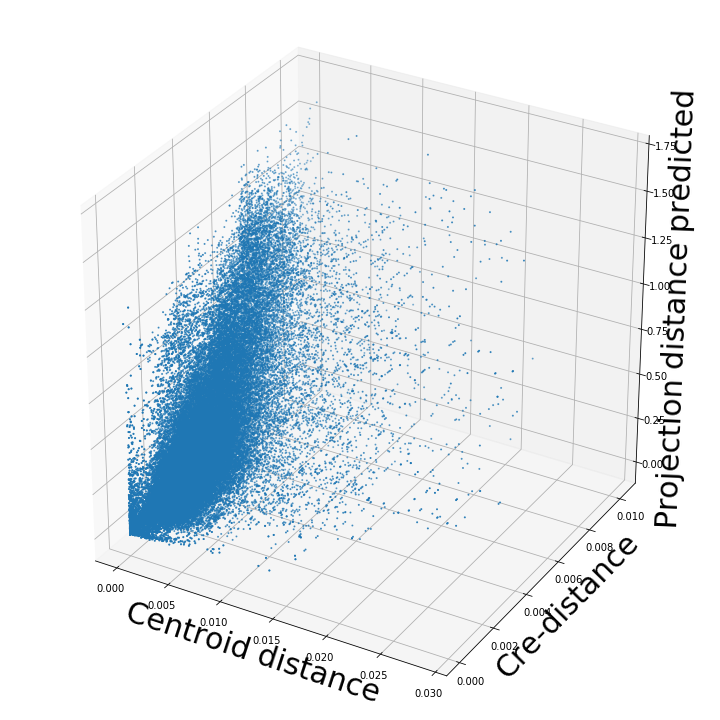
\includegraphics[width = 2.1in]{figs/figsforpres/315_summary_scatter.png}
    %\caption{Isocortex loss distribution}
    \label{fig:my_label} 
    }
    \\
    &
    %\begin{figure}
    %\centering
    \subfloat[]{
    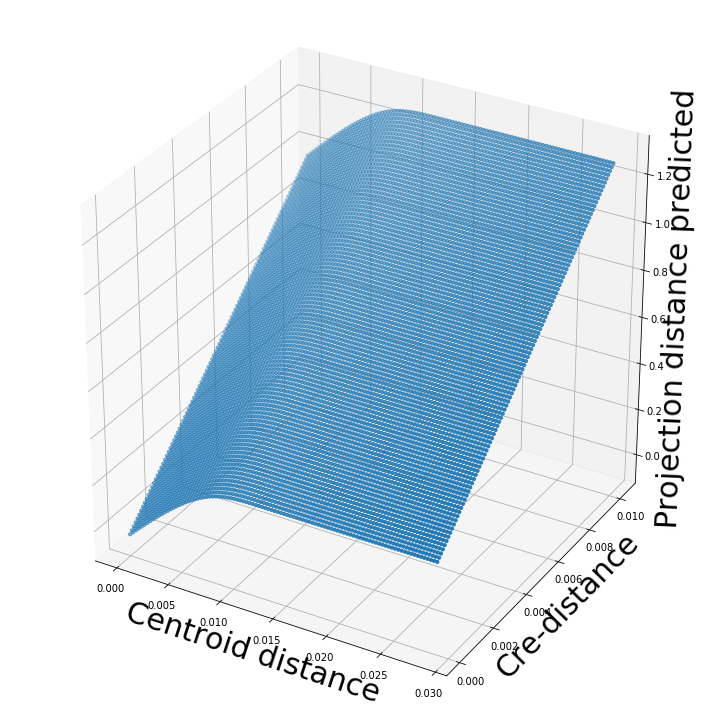
\includegraphics[width = 2.1in]{figs/figsforpres/315_summary_surface.png}
    %\caption{$\hat g$ fit to expected-loss using shape-constrained splines}
    %\captionof{figure}{Caption for image}
    \label{fig:my_label}
    %\end{figure}
    }
    \vspace{1cm}
    \end{tabular}
       
 %  \end{subfigure}
 \end{adjustbox}
 \caption{The Expected-Loss estimator}
 \end{figure}
%\end{figure}
%\end{minipage}
%\end{minipage}
%\end{figure}
%\end{tabular}
\newpage



\section{The expected-loss estimator}
\label{supp_sec:el}
The shape-constrained expected-loss estimator introduced in this paper is, to our knowledge, novel.  It should be considered an alternative method to the classic weighted kernel method. While we do not attempt a detailed theoretical study of this estimator, we do establish the need for the shape constraint in our spline estimator. Though this fact is probably well known, we prove a (slightly stronger) version here for completeness.
%This fact is probably well known, but we prove slightly stronger version of this fact here for completeness.

%The estimated function of distances must be concave, monotonically-increasing, and normalized in order to be a valid distance function on the combined space.  

Given a collection of metric spaces $X_1, ... X_n$ with metrics $d_1 ... d_n$ (e.g. $d_{centroid}, d_cre$), and a function $f: (X_1 \times X_1) ... \times (X_n  \times X_n) = g(d_1(X_1 \times X_1),... d_n(X_n \times X_n))$, then then $f$ is a metric iff $g$ is concave, non-decreasing and $g(d) = 0 \Longleftrightarrow d = 0$.

We first show $g$ satisfying the above properties implies that $f$ is a metric.
\begin{itemize}
    \item The first property of a metric is that $f(x,x') = 0 \Longleftrightarrow x = x'$.  The left implication: $x = x' \implies f(x_1, x_1', ... x_n, x_n') = g(0,....,0)$, since $d$ are metrics.  Then, since $g(0) = 0$, we have that $f(x,x') = 0$. The right implication: $f(x,x') = 0 \implies  d = 0 \implies x = x'$ since $d$ are metrics.
    \item The second property of a metric is that $f(x,x') = f(x',x)$. This follows immediately from the symmetry of the $d_i$, i.e. $f(x,x') = f(x_1, x_1', ... x_n, x_n') = g(d_1(x_1, x_1'), ... d_n(x_n, x_n')) = g(d_1(x_1', x_1), ... d_n(x_n', x_n)) =  f(x_1', x_1, ... x_n', x_n) = f(x',x)$.
    \item The third property of a metric is the triangle inequality: $f(x, x') \leq f(x, x^*) +  f(x^*, x') $.  To show this is satisfied for such a $g$, we first note that $f(x,x') = g(d(x,x')) \leq g(d(x, x^*) + d(x^*, x')) $ since g is non-decreasing and by the triangle inequality of $d$. Then, since $g$ is concave, $g(d(x, x^*) + d(x^*, x')) \leq g(d(x, x^*)) + g(d(x^*, x')) = f(x,x^*) + f(x^*, x')$.
    %or $ f(x_1, x_1', ... x_n, x_n') \leq f(x_1, x_1^*, ... x_n, x_n^*) + f(x_1', x_1^*, ... x_n', x_n^*)$.  To show this is satisfied for such a $g$, we first note $f(x_1, x_1', ... x_n, x_n') = g(d_1(x_1, x_1'),... d_n(x_n ,x_n')) \leq g(d_1(x_1, x_1*) + d_1(x_1', x_1*) ,... , d_n(x_n ,x_n*) + d_n(x_n' ,x_n*))$ since g is non-decreasing and by the triangle inequality on d. Then $g(d_1(x_1, x_1*) + d_1(x_1', x_1*) , ... , d_n(x_n , x_n*) + d_n(x_n' ,x_n*)) < f(x_1, x_1*, ... x_n, x_n*) + f(x_1', x_1*, ... x_n', x_n*)$ since $g$ is concave.
    
    %Lemma: h(a+ b) < h(a) + h(b) for a concave increasing function h.  
%Pf: h(a+b) - h(b) < h(a) - h(0) since rate of increase is decreasing.
\end{itemize}

We then show that $f$ being a metric implies that $g$ satisfies the above properties.
\begin{itemize}
    \item The first property is that $g(d) = 0 \Longleftrightarrow d = 0$. We first show the right implication: $g(d) = 0$, and $g(d) = f(x,x')$, so $x = x'$ (since $f$ is a metric), so $d = 0$. We then show the left implication: $d = 0 \implies x = x'$, since $d$ is a metric, so $f(x,x') = 0,$ since $f$ is a metric, and thus $g(d) = 0$.
    %\item 
    %$f$ is a metric, so $f(x,x') = 0 \Longleftrightarrow x = x'$.  Then, since $f(x,x') = g(d (x,x') )$ which $\implies g(0,\dotsc 0) = 0$ since $g$ is increasing.
    \item The second property is that $g$ is non-decreasing. We proceed by contradiction.
    Suppose g is decreasing in argument $d_1$ in some region $[l, u]$ with $0 < l< u$.
    Then $g(d_1(0, l), 0) \geq g(d_1(0, 0), 0) + g(d_1(0, u), 0) = g(d_1(0, u),0)$, which violates the triangle inequality on f. Thus, decreasing $g$ means that $f$ is not a metric, so $f$ a metric implies non-decreasing $g$.
    \item The final property is that $g$ is concave. We proceed by contradiction. Suppose $g$ is strictly convex. Then there exist vectors $d, d'$ such that $g(d + d')  < g(d) + g(d')$.  Assume that $d$ and $d'$ only are non-zero in the first position, and $d = d(0, x), d' = d(0,x')$.  Then, $f(0,x) + f(0,x') <  f(0,x+ x')$, which violates the triangle inequality on $f$.  Therefore, $g$ must be concave.
\end{itemize}

\section{Decomposing the connectivity matrix}

We utilize non-negative matrix factorization (NMF) to analyze the principal signals in our connectivity matrix.
Here, we review this approach as applied to decomposition of the distal elements of the estimated connectivity matrix $\widehat {\mathcal C}$ to identify $q$ connectivity archetypes.
Aside from the NMF program itself, the key elements are selection of the number of archetypes $q$ and stabilization of the tendency of NMF to give random results over different initialization. 

\subsection{Non-negative matrix factorization}

Given a matrix $X \in \mathbb R_{\geq 0}^{a \times b}$ and a desired latent space dimension $q$, the non-negative matrix factorization is
\begin{eqnarray*}
NMF(X, q) = \arg \min_{W \in \mathbb R_{\geq 0}^{a \times q} ,H_{\geq 0}^{q \times b }} \| (  X  - WH)\|_2^2.
\end{eqnarray*}
NMF creates a useful decomposition since $X$ is in the positive orthant, and PCA cannot not apply.
There is no orthogonality without sparsity.

We note the existence of NMF with alternative norms for certain marginal distributions, but leave utilization of this approach for future work \citep{Brunet2004-gi}.
%The NMF objective function
%\begin{eqnarray*}
%\arg \min_{W \in \mathbb R_{\geq 0} ,H_{\geq 0} } \| (\hat{  \mathcal C}  - WH)\|_2^2
%\end{eqnarray*}
We can also apply a mask $1_M \in \mathbb R^{S \times T}$ of ones and zeros and solve
\begin{eqnarray*}
\arg \min_{W \in \mathbb R_{\geq 0} ,H_{\geq 0} } \| 1_M \odot  ((\hat{  \mathcal C}  - WH))\|_2^2
\end{eqnarray*}
For us, such a mask serves for two purposes.
First, it enables computation of the NMF objective while excluding self and nearby connections.
These connections are both strong and linearly independent, and so would dominate the $NMF$ reconstruction error.
Long range connections are more biologically interesting or cell-type dependent.
Second, it enables cross-validation based selection of the number of retained components.
%$1_{\text{dist}\geq 1500 \mu m}$

\subsection{Cross-validating NMF}

Perhaps surprisingly, cross-validation techniques may also be applied to unsupervised learning problems.
These techniques are somewhat standard, but not entirely well-known, so we review them here, in particular as they apply to the NMF problem.
A NMF model is first fit on a reduced data set, and an evaluation set is held out.
After random masking of the evaluation set, the loss of the learned model is then evaluated on the basis of successful reconstruction of the held-out values.
This procedure is performed repeatedly, with different held out regions and random mask at different dimensionalities $l$, to determine to point past which additional hidden units provide no reconstructive value.

That is, given a matrix $X \in \mathbb R^{S \times T}$ we can decompose $X \sim d(e(X))$ where $e(X)$ is some map that encodes $X$ in a learned representation, and $d$ is the decoding reconstruction map.
In our case, $d$ is simply left multiplication by $W$, and $e$ is the solution of a regularized non-negative least squares optimization problem
\begin{align*}
H := e_W(X) = \arg \min_{\beta} \|X - W \beta\|_2^2.
\end{align*}
%We note 
The form of this solution particularly motivates our cross-validation estimator.

Recall that in supervised learning, the learned model is $Y \sim f(X)$.
Standard cross-validation removes elements of $X$, fits $f$, and then uses the $f$ learned from part of the data to predict $Y$.
A good $f$ will have low error on the training data, and also low error on the test data, indicating that it has not overfit.
Although there is no assumed dichotomy between $X$ and $Y$ in unsupervised learning, for techniques like autoencoders, the above paradigm still applies, i.e., one can still hold out values of $X$.
We can then estimate 
\begin{align*}
\arg \min_{d,e} \widehat E(l(X, d_{X^C}(e_{X^C}(X)))) = \sum_{r=  1}^R l(X_r, d_{X^{C_r}}(e_{X^{C_r}}(X_r)))
\end{align*}
over $R$ random samples of rows of $X$.
However, in our setting, since computing $e(X)$ on the test rows amounts to fitting a non-negative least squares w.r.t. $W$, so the negative effects of an overfit model can simply be optimized away from.
Thus,  the standard solution is to generate uniformly random masks $1_{M(p)} \in \mathbb R^{S \times T}$ where
\begin{align*}
1_{M(p)} (s,t) \sim \text{Bernoulli(p)}.
\end{align*}
%randomly mask $\widehat {\mathcal C}$, we can evaluate the 
Our cross-validation error is then
\begin{align*}
\epsilon_q &= \frac{1}{R} \sum_{r = 1}^R (\|1_{M(p)_r^C} \odot X - \widehat d_q(\widehat e_q (1_{M(p)_r^C} \odot X ))\|_2^2 
\end{align*}
where
\begin{align*}
\widehat d_q, \widehat e_q &= \widehat{\text{ NMF}}(1_{M(p)_r} \odot X, q)).
\end{align*}
The optimum number of components is then
\begin{align*}
    \widehat q = \arg \min_q \epsilon_q.
\end{align*}

\subsection{Stabilizing NMF}

The NMF program is non-convex, and, empirically, individual replicates will not converge to the same optima.
One solution therefore is to run multiple replicates of the NMF algorithm, cluster the resulting vectors.
This approach raises the questions of how many clusters to use, and how to deal with stochasticity in the clustering algorithm itself.
We address this issue through the notion of clustering stability \citep{Von_Luxburg2010-lu}.

The clustering stability approach is to generate $L$ replicas of k-cluster partitions $\{C_{kl} : l \in 1 \dots L\}$ and then compute the average dissimilarity between clusterings
\begin{align*}
\xi_k &= \frac{2}{L(L - 1)} \sum_{l = 1}^{L} \sum_{l'= 1}^{l}  d(C_{kl}, C_{kl'}).
\end{align*}
Then, the optimum number of clusters is 
\begin{align*}
\hat k &= \arg \min_k \xi_k.
\end{align*}
A review of this approach is found in \citet{Von_Luxburg2010-qe}.
Intuitively, archetype vectors that cluster together frequently over clustering replicates indicate the presence of a stable clustering.
For $d$, we utilize the adjusted Rand Index - a simple dissimilarity measure between clusterings.
Note that we expect to select slightly more than the $q$ components suggested by cross-validation, since archetype vectors which appear in one NMF replicate generally should appear in others.
We then select the $q$ clusters with the most archetype vectors - the most stable NMF results - and take the median of each cluster to create a sparse representative archetype.

%http://alexhwilliams.info/itsneuronalblog/2018/02/26/crossval/

\section{Establishing a lower detection limit}

The lower detection limit of our approach is a complicated consequence of our experimental and analytical protocols.
For example, the Nadaraya-Watson estimator is likely to generate many small false positive connections, since the projection of even a single experiment within the source region to a target will cause a non-zero connectivity in the Nadaraya-Watson weighted average.
On the other hand, the complexities of the experimental protocol itself and the image analysis and alignment can also cause spurious signals.
Therefore, it is of interest to establish a lower-detection threshold below which we have very little power-to-predict.
We will then set estimated connectivities below this threshold to zero.
This should make our estimated connectivities more accurate, in particular in the biologically-important sense of sparsity.

The limit-of-detection problem is common in a variety of scientific fields, but statistical methodology is not 
We utilize the zero-inflated adjusted Kendall-$\tau$ statistic

\begin{align*}
    \tau_0 = p_{11}^2 \tau_11 + 2(p_{00} p_{11} - p_{10} p_{01}),
\end{align*}
where \citep{Pimentel2009KendallsTA, Albasi2018-iv}

%\section{Cross-validation for unsupervised learning}












%\section{Data}\label{sec:supp_structure_cre}

%\begin{figure}
%    \centering
%    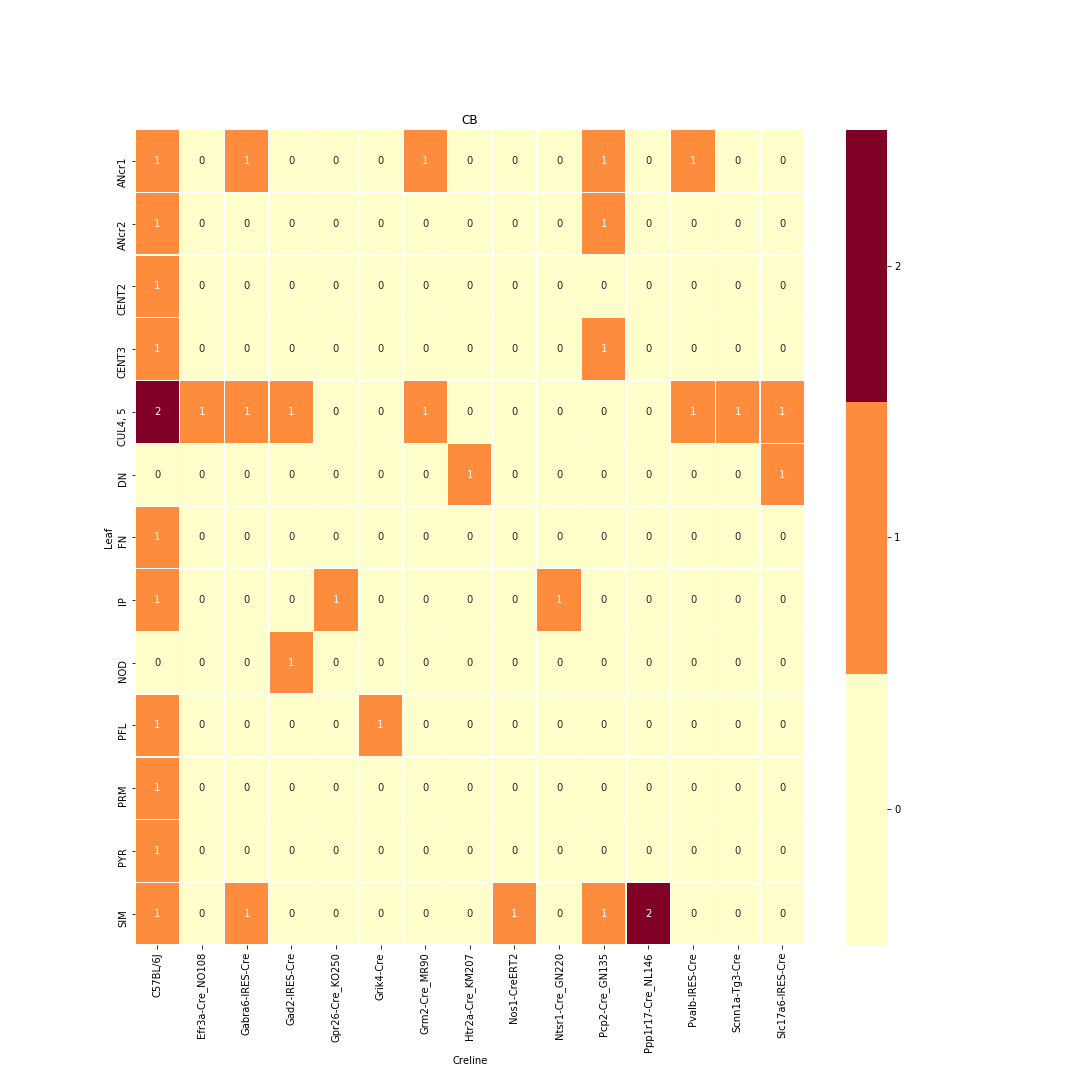
\includegraphics[width = 7in]{figs/CB centroid densityoct12.png}
%    \caption{Caption}
%    \label{fig:my_label}
%\end{figure}


%\section{Model evaluation}
%\label{supp_sec:model-evaluation}



%\begin{table}[]
%    \centering
%    \begin{tabular}{c|c}
%         &  \\
%         & 
%    \end{tabular}
%    \caption{Caption}
%    \label{tab:cross-validation}
%\end{table}

%However, for alternate models, such as the major-structure divided model from \citet{Knox2019-ot}, the potential evaluation set is larger. In order to compare between methods, we therefore restrict to the smallest set of evaluation indices, which is to say, virus-leaf combinations that are present at least twice.  This means that in some cases, our training set exceeds our evaluation set in size. 
